\subsection{Experimentation}

In diesem Unterkapitel werden verschiedene R-Pakete, welche Funktionen für Topic Modeling-Methoden bereitstellen, ausprobiert. Die meisten dieser Pakete werden in \cite{Wiedemann2022-tm-R} angeführt.

Als Datenquelle für die Modelle und Algorithmen wird \textbf{Projekt Gutenberg} herangezogen, ein Online-Archiv für historische Werke. Projekt Gutenberg stellt ein R-Paket zur Verfügung, wessen Verwendung in der Auflistung \ref{list:code-gutenbergr-inst} angeführt wird \cite{gutenbergr}.

\begin{listing}
    \begin{code}{R}
        install.packages("gutenbergr")
        library(gutenbergr)
    \end{code}
    \caption{Installation und Verwendung vom R-Paket "gutenbergr"}
    \label{list:code-gutenbergr-inst}
\end{listing}

Eine Zusammenfassung der wichtigsten Funktionen \cite{gutenbergr}:
\begin{itemize}
    \item Die Funktion \codeinline{R}{gutenberg_works()} gibt eine Liste aller Werke zurück. In der Klammer lassen sich als Parameter Filter wie \codeinline{R}{author=="XY"}, \codeinline{R}{title=="YX"} und \codeinline{R}{gutenberg_id==1234} einsetzen.
    \item \codeinline{R}{gutenberg_works()} gibt unter anderem eine \codeinline{R}{gutenberg_id} der Bücher zurück. Diese verwendet man in der Funktion \codeinline{R}{gutenberg_downloads()}. Diese Funktion kann mehrere IDs sowie sowie Metadaten als Parameter übernehmen, zum Beispiel:
    \\\codeinline{R}{gutenberg_download(c(568, 1204), meta_fields="author")}
\end{itemize}

Die Codezeilen aus der Auflistung \ref{list:code-poe} laden den Text aller Werke vom Author Edgar Allan Poe herunter und werden von allen Modellen verwendet.

\begin{listing}
    \begin{code}{R}
        ## using necessary packages
        library(gutenbergr)
        ## retrieving data from gutenberg
        search <- gutenberg_works(author=="Poe, Edgar Allan")$gutenberg_id
        poe_data <- gutenberg_download(search)$text
    \end{code}
    \caption{Codezeilen zum Download aller Werke von E.A. Poe}
    \label{list:code-poe}
\end{listing}


\subsubsection{Paket \codeinline{R}{textmineR}}

Das Paket \textbf{textmineR} ist einer der modernsten Pakete, welche LDA unterstützen \cite[288]{Wiedemann2022-tm-R}.

Weiters unterstützt es die Modelle LSA und CTM. In Folge werden einfache Prototypen erstellt, für welche man die Datenverarbeitung und deren Einfachheit des Pakets sowie den Output des Modells analysiert.

Das erste Beispiel bzw. Experiment vom Paket \codeinline{R}{textmineR} zeigt die Verwendung mit \textbf{LDA}. Der Code ist in der Auflistung \ref{list:code-textmeineR-lda} angeführt.

Das Ergebnis der letzten Funktion \codeinline{R}{SummarizeTopics(poe_lda)} ist in Abbildung \ref{fig:res-lda-textmineR} zu sehen. An sich tut es das, was es tun soll: Den zehn Topics wurden Wörter zugeordnet. 

Es gibt sogar Daten wie \codeinline{R}{prevalence} und \codeinline{R}{coherence}, welche für Analysezwecke des Modells selbst verwendet werden können. Es gibt jedoch zwei Dinge, die möglicherweise störend sind.

Einerseits wird den Topics bereits ein Label gegeben. Der ganze Sinn dieser Arbeit besteht darin, dass Schüler selbst die Topics benennen. Das ist nicht allzu schlimm, da man diese Spalte entfernen kann.

Was störender ist sind die zwei Spalten mit den Topic-bezogenen Wörtern. Vor allem der Umstand, dass manche Wörter zweimal vorkommen, hilft nicht. In der Dokumentation des Pakets \codeinline{R}{textmineR} steht auch nichts darüber, selbst die Anzahl der Wörter zu setzen, welche angezeigt werden. Das macht dieses Paket ungeeignet für manche Anwendungen, zum Beispiel wenn es einen Slider gibt, mit dem man die Anzahl der Wörter pro Topic bestimmen möchte.

\begin{listing}
    \begin{code}{R}
        ## neccessary packages
        library(textmineR)
        library(stringr)
        ## removing all non-english letters and characters
        ### due to error it is necessary to remove any unknown characters
        poe_data_n <- str_remove_all(poe_data, "[^[\\da-zA-Z ]]")
        ## creating a document term matrix (dtm)
        poe_dtm <- CreateDtm(doc_vec = poe_data_n)
        ## fitting a lda-model with 100 samples of data and 10 topics
        set.seed(123)
        poe_lda <- FitLdaModel(dtm = poe_dtm[1:700,], k = 15, iterations = 250, burnin = 210)

        ergebnis_lda <- SummarizeTopics(poe_lda)
        ergebnis_lda
    \end{code}
    \caption{Anwendungsbeispiel von LDA im Paket textmineR}
    \label{list:code-textmeineR-lda}
\end{listing}

\begin{figure}
    \centering
    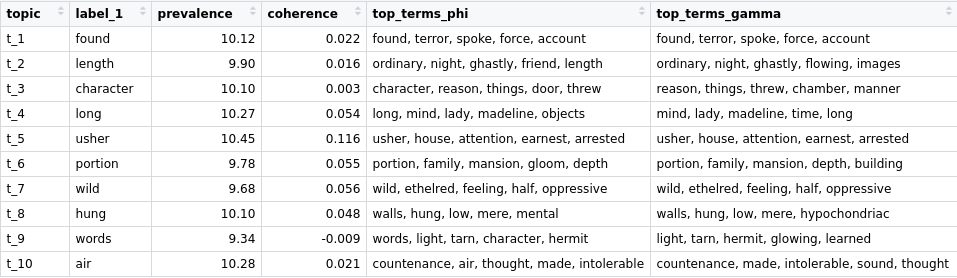
\includegraphics[scale=0.45]{images/dlengsteiner/ergebnis_textmineR_lda_n.png}
    \caption{Ergebnis von LDA (Paket \codeinline{R}{textmineR})}
    \label{fig:res-lda-textmineR}
\end{figure}

Das nächste Beispiel (Auflistung \ref{list:code-textmineR-lsa}) zeigt die Verwendung mit \textbf{LSA} (alle Variablen bis \codeinline{R}{poe_dtm} vom vorherigen Experiment wurden für dieses Experiment ebenfalls verwendet). 

Das zweite Problem von vorher ist hier verstärkt (siehe Abbildung \ref{fig:res-lsa-textmineR}). Es sind nämlich nicht nur ein paar Wörter in den top\_terms-Spalten doppelt veorhanden, sondern es sind alle Wörter betroffen. Je nach Anwendungsfall kann das zu einem Problem werden, vor allem Kombiniert mit der Tatsache, dass man die Anzahl der Wörter pro Topic nicht erhöhen kann.

\begin{listing}
\begin{code}{R}
    set.seed(1234)
    poe_lsa <- FitLsaModel(dtm = poe_dtm, k = 10)
    ergebnis_lsa <- SummarizeTopics(poe_lsa)
    ergebnis_lsa
\end{code}  
    \caption{Anwendungsbeispiel von LSA im Paket textmineR}
    \label{list:code-textmineR-lsa}
\end{listing}

\begin{figure}
    \centering
    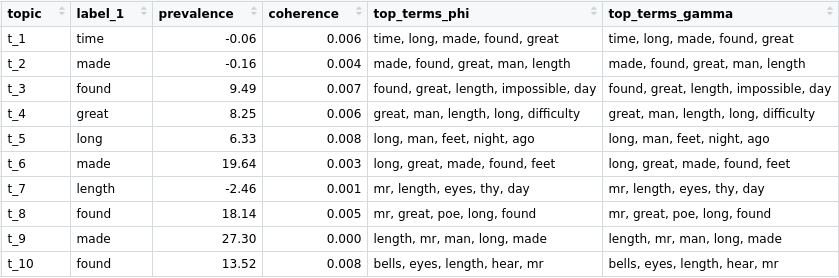
\includegraphics[scale=0.5]{images/dlengsteiner/ergebnis_textmineR_lsa.png}
    \caption{Ergebnis von LSA (Paket \codeinline{R}{textmineR})}
    \label{fig:res-lsa-textmineR}
\end{figure}



\subsubsection{Paket \codeinline{R}{tm}}

Das Paket \codeinline{R}{tm} ist ein sehr mächtiges Paket, welches für Textmining-Zwecke verwendet wird. 
